We start by only considering a single power law operator (out of two in the case of an attractive-repulsive interaction potential $K_{\alpha, \beta}$).
Substituting our ansatz given in \Cref{eq:ansatz} into $\mathcal{Q}^\beta[\rho]$, we obtain
\begin{equation}
  \mathcal{Q}^{\beta}[\rho](x) = \sum_{k=0}^{N-1} \rho_{k} \int_{B_1(\vec{0})} \norm{\vec{x}-\vec{y}}^{\beta} \weight{y}\jacobi{y} \,\dd\vec{y}\,,
  \label{eq:theorem216-in-derivation}
\end{equation}
luckily containing the integral evaluated in \Cref{thm:theorem216}.

We are now interested in a numerical representation of the operator $\mathcal{Q}^\beta$ acting on the function $\rho \in \functionspace$, so an equivalent (linear) operator $Q^\beta: \R^N \to \R^N$ acting on the coefficients $\rho_k \in \R,\, k = 0, ..., N-1$.
As every finite-dimensional linear operator must have a matrix representation, we look for a $Q^\beta \in \R^{N \times N}$ such that
$$\mathcal{Q}^\beta[\rho](\vec{x}) = \jacobivec{x} \cdot Q^\beta \vec{\rho}\,,$$
where $\jacobivec{x} \in \R^N$ is the vector of radial Jacobi polynomials $P^{(a, b)}_0(x)$, $P^{(a, b)}_1(x)$, ..., $P^{(a, b)}_{N-1}(x)$ evaluated at $2\norm{\vec{x}}^2 - 1$ as introduced in and after \Cref{def:jacobi-polynomials}.
Note that in the context of linear combinations of Jacobi polynomials, we will use zero-based indexing for vectors and matrices due to the convention that the first orthogonal polynomial is usually denoted by $p_0(x) = 1$, in line with $\deg(p_k) = k$.

Based on the three-term recurrence relationship (cf. \Cref{thm:three-term-recurrence-relationship}), one can even determine an explicit relationship between the coefficients in the Jacobi expansion by considering the Jacobi matrix (cf. \Cref{remark:jacobi-matrix}).
We use this recurrence relationship in our implementation to significantly speed up the construction of the operator (cf. \Cref{sec:runtime-analysis}).
The recurrence coefficients used are due to \cite{2021-arbitrary-dimensions} and \cite{2023-olver-equilibrium-measures-jl}.

% TODO: this section has weird indexing (start at 0 or 1?) and needs some work.
Therefore, starting from \Cref{eq:theorem216-in-derivation}, we obtain
\begin{align*}
  \mathcal{Q}^\beta[\rho](\vec{x}) & = \sum_{k=0}^{N-1} \rho_k \mathcal{Q}^\beta[wP_k](\vec{x}) = \sum_{k=0}^{N-1} \rho_k \sum_{j=0}^{N-1} q^{\beta}_{kj} \jacobi{x} \\
                                   & = \sum_{j=0}^{N-1} \sum_{k=0}^{N-1} \rho_k q^{\beta}_{kj} \jacobi{x}\,,
\end{align*}
which we will rewrite in matrix-form,
\begin{align*}
  \mathcal{Q}^\beta[\rho](\vec{x}) & = \vec{P}(\vec{x}) \cdot
  \begin{pmatrix}
    \sum_{k=0}^{N-1} \rho_k q^{\beta}_{k,1} \\
    \vdots                                  \\
    \sum_{k=0}^{N-1} \rho_k q^{\beta}_{k,N}
  \end{pmatrix} = \vec{P}(\vec{x}) \cdot
  \underbrace{
    \begin{pmatrix}
      q^{\beta}_{00}    & \dots  & q^{\beta}_{0,N-1}   \\
      \vdots            & \ddots & \vdots              \\
      q^{\beta}_{N-1,0} & \dots  & q^{\beta}_{N-1,N-1} \\
    \end{pmatrix}
  }_{=: Q^\beta}
  \begin{pmatrix}
    \rho_0 \\
    \vdots \\
    \rho_{N-1}
  \end{pmatrix}                                                              \\
                                   & = \jacobivec{x} \cdot Q^\beta \vec{\rho}
\end{align*}
where we use $\vec{P}(\vec{x}) = \jacobivec{x}$ as a shorthand giving us the form of the operator matrix.
Its first row, the set of coefficients for the constant Jacobi polynomial $P_0^{(a,b)}$ of each expansion of $Q^\beta$, weighted by the solution coefficients, adds up to the total energy $E$ (coefficient of the constant polynomial).
All remaining rows of $Q^\beta$ contain coefficients for polynomials of degree at least 1, so their weighted contributions must add up to 0 in order for the total energy $\tilde{E}(\vec{x})$ to remain constant.

For the attractive-repulsive interaction potential $K_{\alpha,\beta}$, because each column consists of an expansion of the Jacobi polynomials, we have $q^{\beta}_{0k} = I_{m,k}^{\alpha,\beta}$.

\begin{figure}[H]
  \centering
  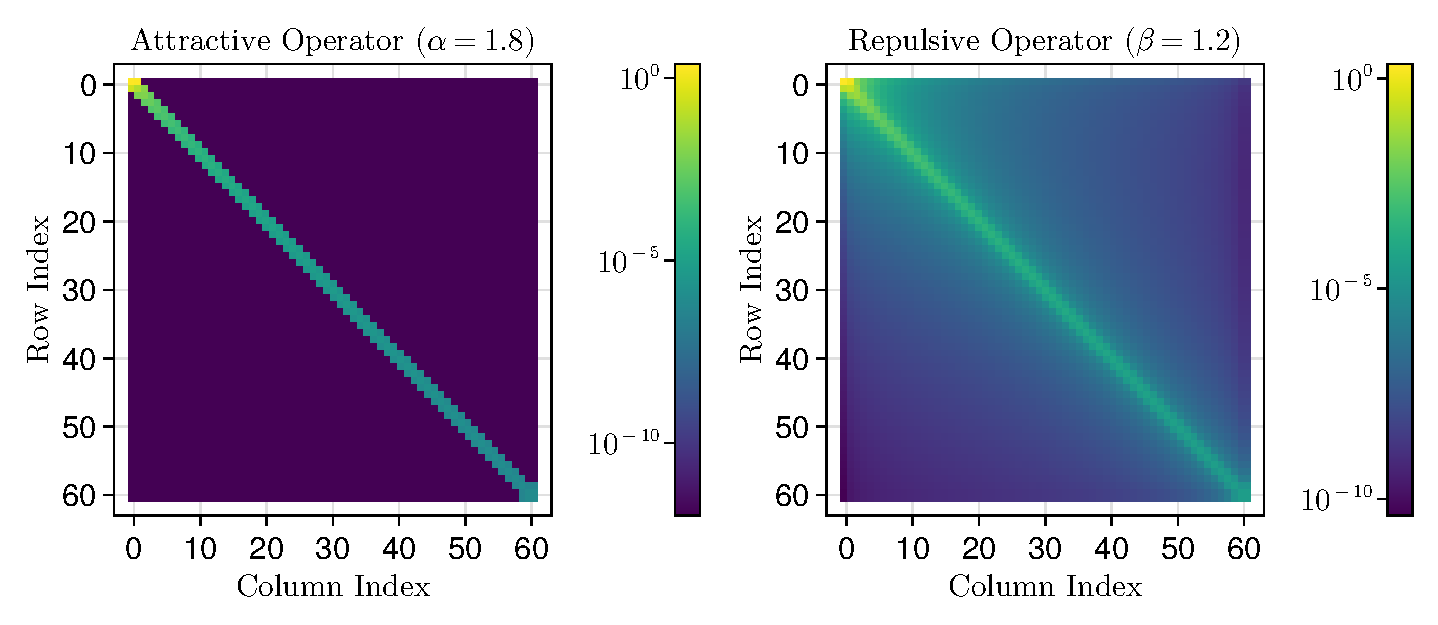
\includegraphics[width=\linewidth]{results/attrep/attractive-repulsive-operators.pdf}
  \caption[Attractive and repulsive operators.]{The attractive and repulsive operators (matrices) as given in \Cref{def:power-law-operator}, the matrix values are shown in a $\log_{10}$ colour scale. Due to the choice of basis, the attractive operator is exactly banded. The repulsive parameter is only approximately banded, which the spy plots effectively demonstrate.}
  \label{fig:attractive-repulsive}
\end{figure}

The exact bandedness of the attractive operator in \Cref{fig:attractive-repulsive} is due to the three-term recurrence relationship of the Jacobi polynomial basis (cf. \Cref{thm:three-term-recurrence-relationship} and \Cref{def:jacobi-polynomials}).
